\documentclass[12pt,a4paper]{article}

%\usepackage{german}
\usepackage{a4wide}
\usepackage{graphicx}
\usepackage{amssymb}
\usepackage{amsmath}
\usepackage{ae,aecompl}

\pagestyle{empty}
\setlength{\parindent}{0pt}
\renewcommand{\labelenumi}{\alph{enumi})}
\renewcommand{\labelenumii}{\roman{enumii})}

\newcommand{\aufg}[1]{\vspace{4mm}{\bf\underline{Problem #1:}}\vspace{3mm}}

\begin{document}
\vspace*{-3cm}
\begin{center}
{\large\bf GLoBES Tutorial: Finding Degeneracies}\\[0.3cm]
GLoBES workshop in Heidelberg, Germany, January 24-26, 2007
\end{center}
\vspace*{2mm}

Walter\ Winter \hfill January 25, 2007

\bigskip
\hrule
\vspace*{4mm}

{\small
In this advanced-level tutorial, we illustrate several techniques for discrete degeneracy localization in GLoBES (General Long Baseline Experiment Simulator). In order to include correlations as well, the unused parameters are usually marginalized/minimized over for a given set of simulated parameters. In principle, one can include all degenerate solutions in GLoBES by a complete scan of the parameter space with {\tt glbChiSys}. However, such a ``grid-based'' approach takes $g^d$ steps, where $g$ is the number of steps in one dimension (such as $\theta_{13}$), and $d$ is the dimension of the parameter space (typically $d=6$ for neutrino oscillations). For example, for 
$g=20$ steps in one direction, $20^6 = 6.4 \cdot 10^7$ evaluations of the systematics $\chi^2$
would be necessary, costing many hours of CPU time on a modern computer -- and this is only
for one set of input parameters. Therefore, GLoBES provides the concept of local minimization: Instead of scanning the complete parameter space, most of which is uninteresting because of a too large $\chi^2$,
a minimizer is started at the position of an ``educated guess'' and runs into the local minimum to include the correlations with the other parameters.
This reduces the computational effort to about $n \times 1 \, 000$ evaluations of the systematics $\chi^2$, where $n$ is the number of discrete degeneracies. For example, for $n=8$, the computational effort can be reduced from several hours to a few seconds. Since the local minimizer may end up in the wrong minimum if started too far away from the actual solution, finding a proper educated guess for the discrete degeneracies is crucial for this approach. Therefore, most of this tutorial deals with {\em methods to find an educated guess}. Note that the chosen examples do not represent the standard level of sophistication needed to use GLoBES, such as to simulate superbeams. They are chosen from a large set of calculations to illustrate cases where the straightforward methods fail.
}

\vspace*{0.5cm}

\subsubsection*{Finding the $\boldsymbol{\mathrm{sgn}(\Delta m_{31}^2)}$-degeneracy at T2HK} 

\aufg{1} {\bf Warm-up}

In this tutorial, all programs are labeled {\tt deg\_tut\_n.c}, where {\tt n} is the problem number.
In every problem, the program, which we have provided for you, illustrates a straightforward solution. As you will see, we have chosen examples where the straightforward approach will fail. Familiarize yourself with the source code, compile the program with {\tt make deg\_tut\_n}, and run it with {\tt ./deg\_tut\_n}. You will see some additional information on screen while the program is executed. The output is, as a standard, written into a file named {\tt tutn.dat}, {\tt n} being the problem number again. Take a look at the output, which is a simple two-column file, with the editor or plot program of your choice. For example, start {\tt gnuplot} and enter {\tt plot "tutn.dat" with lines}.
%
As the next step, we will describe a possible solution to the problem, and is up to you to implement it in the given program file. We will demonstrate how the output should look like, but we will not provide a specific program code for the solution. 

\vspace*{3mm}

Let's try that. In this example, we want to find the minimum $\chi^2$ at the $\mathrm{sgn}(\Delta m_{31}^2)$-degeneracy for T2HK. This values describes the sensitivity to the normal hierarchy as function of $\mathrm{log}( \sin^2 2 \theta_{13})$. We compute it as function of the simulated (true) $\mathrm{log}( \sin^2 2 \theta_{13})$ for the simulated $\delta_\mathrm{CP}=3 \pi/2$ in the program {\tt deg\_tut\_1.c}.
Try to follow the procedure above. This is what your result should look like: 

\begin{center}
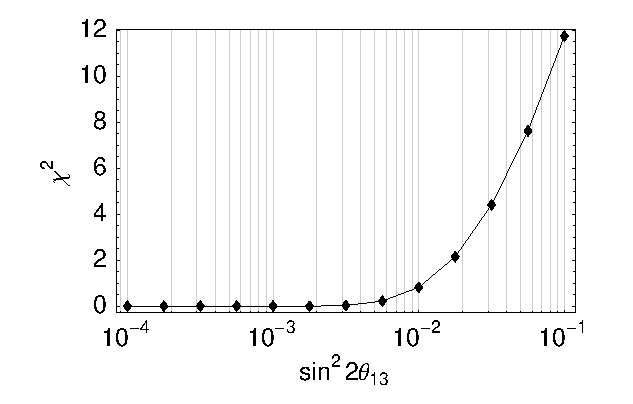
\includegraphics[height=4.5cm]{problem1}
\end{center}

The result is a smooth $\chi^2$, and the straightforward algorithm seems to work. Nothing to do here - but just wait, until we change $\delta_\mathrm{CP}$ in the next problem.

\aufg{2} {\bf Using analytical knowledge}

In this problem, we simply change $\delta_{\mathrm{CP}}$, {\it i.e.}, we compute the $\chi^2$ for the normal mass hierarchy sensitivity as function $\mathrm{log}( \sin^2 2 \theta_{13})$ for the simulated $\delta_{\mathrm{CP}}=\pi/8$. The result is the solid curve in the following plot:

\begin{center}
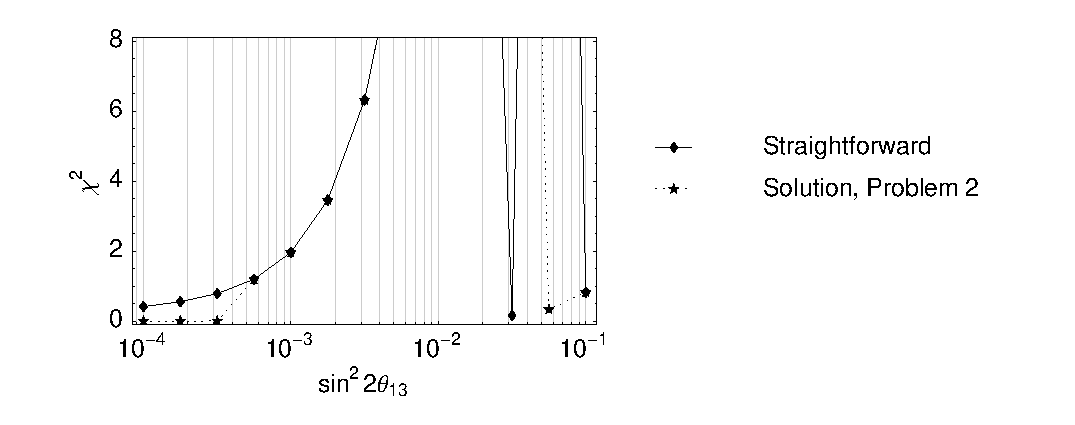
\includegraphics[height=5cm]{problem2}
\end{center}

Obviously, the calculated $\chi^2$ is much to large for the experiment considered: T2HK cannot measure the mass hierarchy very well because of the rather short baseline. The reason for the poor performance of our method is the contribution from both appearance and disappearance channels used in this experiment. In certain regions of the parameter space, the disappearance information is at least comparable to the appearance $\chi^2$, which means that one cannot rely on one specific topology (such as of the appearance channel). The educated guess for the minimizer is obviously not good enough.

\vspace*{3mm}

\underline{Possible improvement:}
 For very small $\theta_{13}$, the appearance rate in T2HK will be almost zero. Therefore, the topology is determined by the disappearance channel. 

Fortunately, one can in this case obtain a very simple guess for the location of the degeneracy in $\Delta m_{31}^2$ (see, {\it e.g.}, Ref.~\cite{deGouvea:2005mi}):
\begin{equation}
(\Delta m_{31}^2)^- = - (\Delta m_{31}^2)^+ + 2 \, \Delta m_{21}^2 \, \cos^2 \theta_{12} \, .
\end{equation}
Use this value to start the minimizer there. As you see in the plot (dashed curve), this works very well for small $\theta_{13}$, but it fails for larger $\theta_{13}$ where the appearance channel adds information. In the next
problem, we will use a different method, which is more successful in this particular example. However, note that analytical knowledge can also be used for the appearance channel and for other problems. We have just restricted ourselves to the simplest example we could think of.

\aufg{3} {\bf Tracking algorithm}

Let us now improve the solution from last example by using a different method.

\vspace*{3mm}

\underline{Possible solution:} Assume that the straightforward approach works in a part of the parameter space, and we find a solution there which is good enough. A {\em tracking algorithm} can then use the output from {\tt glbChiAll} (local minimum, returned as the second parameter) as the input for the next minimization if the points are not too far apart from each other. In this case, the parameter space is ``adiabatically'' changed. Use, for example, $\theta_{13}=0$ as a starting guess and, from there, move gradually upward in $\theta_{13}$. 
The result should then resemble the dashed curve in the following figure:
\begin{center}
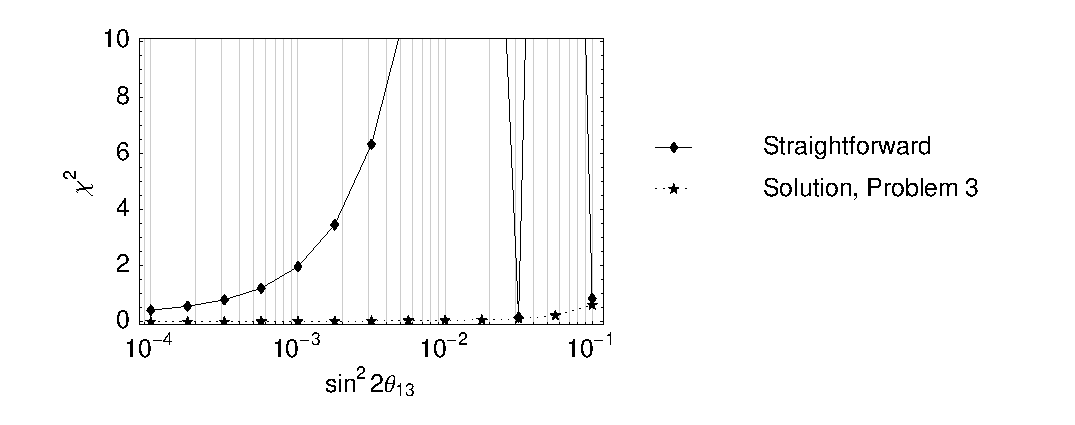
\includegraphics[height=5cm]{problem3}
\end{center}
In this particular case, it is a very good solution. If you scan the parameter space in the (true) $\delta_\mathrm{CP}$-direction (and other true parameter directions)
continously, you will find cases where the method fails for small $\theta_{13}$. Combine then the solutions
of problem~2 and problem~3, and you will have a working algorithm.

\subsubsection*{Locating the intrinsic $\boldsymbol{(\delta_\mathrm{CP},\theta_{13})}$-degeneracy at a neutrino factory} 

\aufg{4} {\bf Pre-scanning a parameter sub-space}

We now consider a different experiment. A neutrino factory typically faces the intrinsic degeneracy
problem in a part of the parameter space. In this example, we compute the $\sin^2 \theta_{13}$ precision, {\it i.e.}, the $\chi^2$ as function of the fit $\sin^2 \theta_{13}$ for a given set of simulated values. We project onto the $\sin^2 \theta_{13}$-axis, because we want to read off the precision of $\sin^2 \theta_{13}$ including all correlations. In order to start the minimizer, we use the set of true/simulated values as an educated guess for the minimizer. We obtain the solid curve in the following figure:

\begin{center}
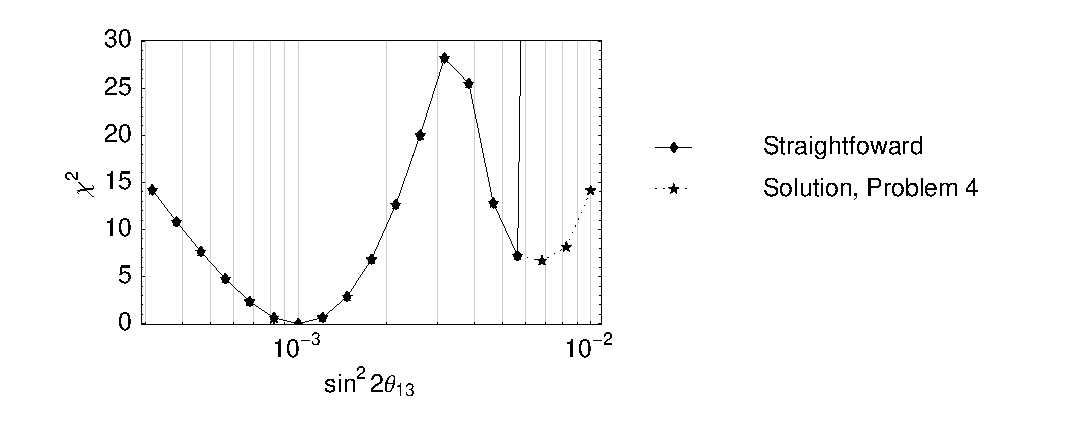
\includegraphics[height=5cm]{problem4}
\end{center}

Obviously, the $(\delta_\mathrm{CP},\theta_{13})$-degenerate solution on the right is not located properly. The reason is that the minimizer ends up in the local minimum corresponding to the best-fit point, whereas the degeneracy is located at a different value of $\delta_\mathrm{CP}$.

\vspace*{3mm}

\underline{Possible solution:}
For each $\sin^2 2 \theta_{13}$, use {\tt glbChiSys} to pre-scan the parameter space in the $\delta_{\mathrm{CP}}$ direction only. Since {\tt glbChiSys} is very fast, one can just scan the $\delta_{\mathrm{CP}}$-direction for the local minimum in the $\delta_{\mathrm{CP}}$ direction, and then use this
as a guess for the minimizer (such as using 50 steps from $0$ to $2 \pi$). This guess does not include the full correlation, but it exploits the dominant effect in an efficient manner. The full correlation is then obtained by the following run of {\tt glbChiTheta13}. The result is the dashed curve in the above figure.

\subsubsection*{Octant $\boldsymbol{(\theta_{23},\pi/2-\theta_{23})}$-degeneracy } 

\aufg{5} {\bf Manual scan of a sub-space}

Locating the octant degeneracy is a computationally equivalent to the ability of an experiment to exclude the
other (``wrong'') octant. Naturally, one would use 
$\pi/2 - \theta_{23}$ as a guess for the starting point of the minimizer.
The octant degeneracy is especially tricky from the computational point of view 
for $\theta_{23}$ very close to maximal mixing: In this case, the local minimizer tends to end up
in the best-fit octant -- there is no barrier for preventing it from doing so. We illustrate this in this problem using T2HK, which has, as a standalone experiment without atmospheric data, a very weak octant resolution potential. 
For example, for $\sin^2 2 \theta_{13}=0.1$, we obtain the solid curve in the following figure as function of the simulated $\sin^2 \theta_{23}$:
\begin{center}
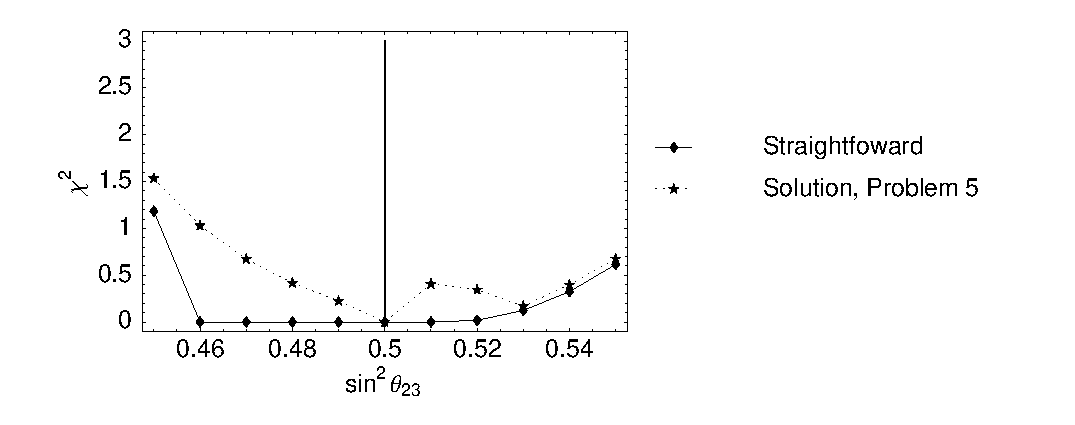
\includegraphics[height=5cm]{problem5}
\end{center}
As the algorithm tells you when you run it (see source code), the minimizer ends up in the wrong octant
for four points left and two points right adjacent to the vertical line (note that at the best-fit solution, $\chi^2 = 0$). So how can we prevent it from doing so? One possibility is to add an external constraint on $\theta_{23}$. However, this does not guarantee ending up in the targeted octant. In addition, a too high external precision in this constraint will make the $\chi^2$ artificially higher. In this and the next problem, we therefore discuss two possibilities which end up in the right octant for sure.
 
\vspace*{3mm}

\underline{Possible solution:}
Instead of minimizing over all parameters simultaneously, scan the $\theta_{23}$-direction separately and
use {\tt glbChiNP} with a user-defined projection to marginalize over the other parameters (keeping $\theta_{23}$ fixed). Therefore, we split the marginalization procedure in a grid-based and local minimization process. For example, for the simulated $\sin^2 \theta_{23} = 0.45$, scan the fit $\sin^2 \theta_{23}$ from $0.5$ to $0.6$ in steps of $0.005$ (or larger steps, if too slow), and minimize over the other parameters for each $\sin^2 \theta_{23}$. Choose the minimum $\chi^2$ from the $\theta_{23}$ scan. Make sure to cover a large enough range for the $\theta_{23}$ scan in the wrong octant. Using this procedure, it is obvious that one cannot end up in the unwanted octant. As a result, you should find the dashed curve in the above figure (for a stepsize of $0.005$). However, as you can check, the result somewhat depends on the grid width/stepsize (which explains the discrepancy for the points ending up in the correct octant). 
For a precision calculation, many steps in $\theta_{23}$ are required (or interpolation techniques in the $\theta_{23}$ direction). In addition, the procedure is extremely slow. 

\aufg{6} {\bf Using Schwetz-priors} (requires GLoBES 3.0 or higher!)

Here we will use a more advanced and very fast approach to the last problem, which is named
after its inventor Thomas Schwetz. It requires GLoBES 3.0 or higher and uses user-defined
priors. However, you will not need any particular knowledge about the implementation: The
example {\tt deg\_tut\_6.c} already defines a standard prior for you. You will only need
to modify the prior where indicated to include the solution.

\vspace*{3mm}

\underline{Possible solution:}
Add a very large value to the $\chi^2$ if the minimizer ends up in the wrong octant. This can be
done with a user-defined prior, which is a function of the oscillation parameters only to be added to the $\chi^2$ {\em before} the oscillation parameter marginalization.  Modify the already implemented user-defined prior function where marked in the code.  Use the {\tt central\_values} to find out
which the right and wrong octant is. Use {\tt in} to extract the tested $\theta_{23}$ and compare it
to the one from {\tt central\_values}. If in the unwanted octant, add a very large number to the $\chi^2$.

As a result, you should find the following dashed-dotted curve with triangles:
\begin{center}
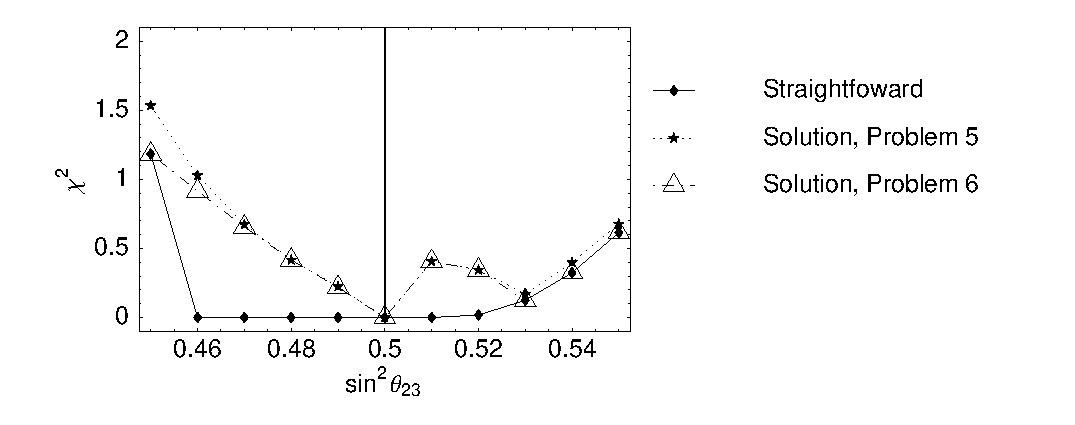
\includegraphics[height=5cm]{problem6}
\end{center}
As you can easily see, the procedure reproduces the correct solutions from the ``straightforward'' curve, but it does not fall in the unwanted octant in the few points close to the vertical line. 

\subsubsection*{Advanced topic: Eight-fold degeneracy}

%\aufg{8} {\bf Pitfalls}

\aufg{7} {\bf Using iso-rate curves} (homework: requires extensive programming!)

In practice, one wants to have a stable and reliable tool for discrete degeneracy localization.
Unfortunately, such a tool depends on the topology and therefore on the experiment.
A typical very sophisticated experiment with all degeneracies being relevant, is a neutrino factory at a baseline of about $2 \, 000 \, \mathrm{km}$ to $4 \, 000 \, \mathrm{km}$. In the literature, the degeneracies
are defined by equal probabilities for both neutrinos and antineutrinos
\begin{equation}
P_{e \mu} (\boldsymbol{\eta_\mathrm{best-fit}}) = P_{e \mu} (\boldsymbol{\eta'}) \, , \quad  P_{\bar{e} \bar{\mu}}(\boldsymbol{\eta_\mathrm{best-fit}}) = P_{\bar{e} \bar{\mu}}(\boldsymbol{\eta'})\, 
\end{equation}
at an oscillation parameter point $\boldsymbol{\eta'}$ and the best-fit value $\boldsymbol{\eta_{\mathrm{best-fit}}}$ (see, {\em e.g.}, Ref.~\cite{Barger:2001yr}).
In principle, one can use analytical knowledge to find all such points $\boldsymbol{\eta'}$ corresponding to the different discrete degeneracies. However, for an experiment using spectral information, the dominating effect will we a weighted average over different energies including the convolution with cross sections, flux, {\em etc.} Therefore, in practice, two different methods turn out to be very efficient:  
\begin{enumerate}
\item
 Winter's method: Use {\tt glbTotalRuleRate} to obtain the total event rates for the neutrino and antineutrino appearance
channels. Plot the curves with equal total rate in the $\sin^2 2 \theta_{13}$-$\delta_{\mathrm{CP}}$-plane for both neutrinos and antineutrinos using the same rates as in the best-fit point. The curves will intersect at the intrinsic degeneracy (if it all). Plot the same curves for the same rates with $\mathrm{sgn}(\Delta m_{31}^2)$ flipped. Again you will find a maximum of two intersection points. Now do the same for $\pi/2 - \theta_{23}$ flipped, and for  $\mathrm{sgn}(\Delta m_{31}^2)$ combined with $\pi/2 - \theta_{23}$ flipped (mixed degeneracy). You will find at most two more intersection points in each case.
The results should look somewhat like this, where the best-fit point is not marked (the marks correspond to the points where the discrete degeneracies are located according to this specific algorithm):
\begin{center}
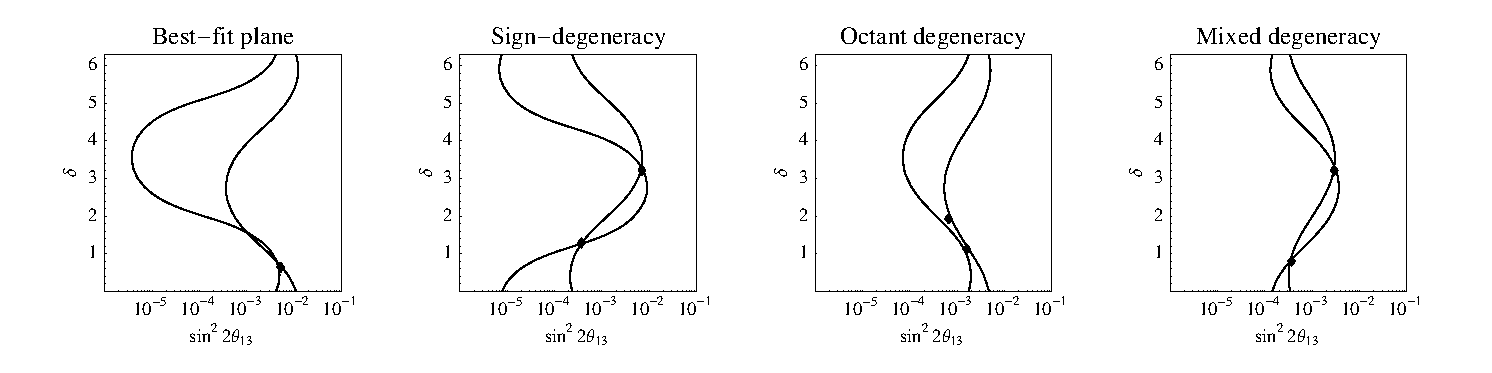
\includegraphics[width=0.95\textwidth]{ircurves}
\end{center}
 Altogether, there is a maximum of eight intersection points in the $\sin^2 2 \theta_{13}$-$\delta_{\mathrm{CP}}$-plane, one of which is the best-fit point. These points can be using as starting points of the minimizer to locate the eight-fold degeneracy.
\item
 Huber's method:
 Pre-scan the $\chi^2$ in the $\sin^2 2 \theta_{13}$-$\delta_{\mathrm{CP}}$-plane for the cases described in~a). Find the local minimum which is separated from the best-fit solution. This method is similar to a), but it uses the $\chi^2$ instead of the total event rate. 
\end{enumerate}

\bibliographystyle{apsrev}
\bibliography{references}

\end{document}
